\documentclass[10pt,compress]{beamer}
%\documentclass[10pt,compress,draft]{beamer}
\mode<presentation>
\usepackage{graphicx}
%\usepackage{beamerthemesplit}
\usepackage[ansinew]{inputenc}
%\usepackage[spanish]{babel}
\usepackage{amsmath,amssymb}
\usepackage{eqlist}
\usepackage{amsfonts} % Simbolos matematicos
\usepackage{amsthm} %Enunciados predefinidos y demostraciones
\usepackage{bbm}
\usepackage{enumerate}
\usepackage[dvips]{epsfig} %Incluir figuras .eps
\usepackage{epsf}%Incluir figuras .eps
\usepackage{eurosym}
\usepackage{subfigure}
\usepackage{graphicx}
\usepackage{multirow}

\useoutertheme[footline=authortitle]{miniframes}
\useinnertheme{circles}
\usepackage{multirow}
\usepackage{animate}
\usepackage{booktabs}
\usepackage{multirow}
\usepackage{siunitx}

\usepackage{chicago}%,e:/latex/psfrag

%%%%%%%%%%
%    1   %
%%%%%%%%%%
\title[Multidimensional Scaling for Big Data\qquad{} MESIO  \qquad{} \insertframenumber %/54]
%/\inserttotalframenumber]
/\pageref{last_page}]
{\LARGE Multidimensional Scaling for Big Data}
\author[Cristian Pach\'on Garc\'ia]{{
   \large Cristian Pach\'on Garc\'ia \\
    \small Advisor: Pedro Delicado Useros
  }
\\
%{\small January 2019}
}
\date{\today}

\usepackage{Sweave}
\begin{document}
\Sconcordance{concordance:simulationV2.tex:simulationV2.Rnw:%
1 46 1 1 0 92 1}


\frame{\titlepage}


\frame{\scriptsize{\tableofcontents} }
\AtBeginSubsection[]
{
  \begin{frame}<beamer>
    \frametitle{}
    \scriptsize{\tableofcontents[currentsection,currentsubsection]}
  \end{frame}
}

\AtBeginSection[]
{
  \begin{frame}<beamer>
   \frametitle{}
    \scriptsize{\tableofcontents[currentsection,currentsubsection]}
  \end{frame}
}

%%%%%%%%%%%%%%%%%%%%%%%%%%%%%%%%%%%%%%%%%%%%%%%%%%%%%%%%
\section{Introduction}

\frame{\frametitle{Divide and Conquer MDS}
  \centering
  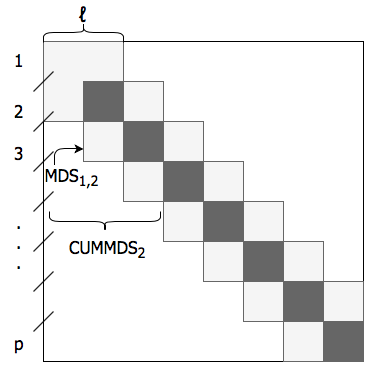
\includegraphics[width=\textwidth,height=0.8\textheight,keepaspectratio]{./images/div_conq_alg.png}
  
}


\frame{


\begin{table}
  \begin{tabular}{rr|rr|rr|rr}
    \hline
     \multicolumn{2}{r|}{} & 
      \multicolumn{2}{c|}{Div. Conq.} & 
       \multicolumn{2}{c|}{Fast} &
       \multicolumn{2}{c|}{Gower}\\
      sample\_size & n\_dim & $\overline{\sqrt{\phi}}$ & $\widehat{\mbox{bias}}$  & $\overline{\sqrt{\phi}}$ & $\widehat{\mbox{bias}}$ & $\overline{\sqrt{\phi}}$ & $\widehat{\mbox{bias}}$\\
      \hline
      $10^3$ & 10  & 14.98 & -0.02 & 15.85 & -0.15 & 15.05 & 0.05  \\ 
      $10^3$ & 100  & 15.03 & 0.03 & 15.01 & 0.01 & 15.02 & 0.02  \\ 
      $3 \cdot 10^3$ & 10  & 15.00 & -0.00 & 14.91 & -0.09 & 14.04 & -0.06  \\ 
      $3 \cdot 10^3$ & 100  & 14.96 & -0.04 & 15.10 & 0.10 & 15.04 & 0.04  \\ 
      $5 \cdot 10^3$ & 10 &  14.99 &  -0.01 & 14.96 & -0.04 & 14.98 & -0.02  \\ 
      $5 \cdot 10^3$ & 100 &  14.99 & -0.01 & 15.03 & 0.03 &15.02 & 0.02  \\ 
      $10^4$ & 10  & 14.99 & -0.01 & 14.33 & -0.67  & 14.99 & -0.01\\ 
      $10^4$ & 100  & 14.99 & -0.01 & 15.09 & 0.09 & 15.06 & 0.06\\ 
      $10^5$ & 10  & 14.99 & -0.01 & 15.00 & 0.0 & 15.04 & 0.04  \\ 
      $10^5$ & 100  & 14.99 & -0.01 & 15.00 &0.0 & 14.97 & -0.03  \\ 
      $10^6$ & 10  & 14.98 & -0.02 & 14.86 & -0.14 & 14.98 & -0.02  \\ 
      $10^6$ & 100  & 14.99 & -0.01 & 14.90 & -0.10 & 14.90 & -0.10 \\ 
    \bottomrule
  \end{tabular}
\end{table}


}

%\begin{table}[ht]
%\centering
%\begin{tabular}{rrrrrr}
% sample\_size & n\_dim & n\_main\_dim & $\overline{\sqrt{\phi}}$ & $\widehat{\mbox{bias}}$ & %$\widehat{\mbox{MSE}}$ \\ 
%  \hline
%  $10^3$ & 10 & 1 & 14.98 & -0.02 & 0.03 \\ 
%  $10^3$ & 100 & 1 & 15.03 & 0.03 & 0.11 \\ 
%  $3 \cdot 10^3$ & 10 & 1 & 15.00 & -0.00 & 0.00 \\ 
%  $3 \cdot 10^3$ & 100 & 1 & 14.96 & -0.04 & 0.16 \\ 
%  $5 \cdot 10^3$ & 10 & 1 & 14.99 &  -0.01 & 0.02 \\ 
%  $5 \cdot 10^3$ & 100 & 1 & 14.99 & -0.01 & 0.01 \\ 
%  $10^4$ & 10 & 1 & 14.99 & -0.01 & 0.01 \\ 
%  $10^4$ & 100 & 1 & 14.99 & -0.01 & 0.00 \\ 
%  $10^5$ & 10 & 1 & 14.99 & -0.01 & 0.01 \\ 
%  $10^5$ & 100 & 1 & 14.99 & -0.01 & 0.01 \\ 
%  $10^6$ & 10 & 1 & 14.98 & -0.02 & 0.03 \\ 
%  $10^6$ & 100 & 1 & 14.99 & -0.01 & 0.01 \\ 
%   \hline
%\end{tabular}
%\caption{Estimator, $\widehat{\mbox{bias}}$ and $\widehat{\mbox{MSE}}$ for 
%        scenarios with one main dimension $\lambda = 15$ for 
%        \textit{Divide and Conquer MDS}.}
%\label{mse_divide_one_dimensions}
%\end{table}
%

\end{document}


